\let\cleardoublepage\clearpage
\chapter{Introduction}
\label{chapter:Introduction}


\textit{"The only truly secure system is one that is powered off, cast in a block of concrete 
and sealed in a lead-lined room with armed guards."
\textemdash  \textbf{ Gene Spafford}} \smallskip

According to the ultimate security vulnerabiltiy datasource CVE details~\cite{cve:details},
there are 2082 vulnerabilities related to information exposure. Among many Information 
Flow(IF) weaknesses, Information exposure is one of the serious issues.
This kind of weaknesses can exist in the code, without breaking anything, yet
providing some confidential information to the attacker 
who wishes to exploit the system. Information exposure bugs could be introduced
at different stages of software development. During design, architecture 
or coding phase 
can expose critical information and lead to strange program behavior. Therefore
care should be taken to test the software thoroughly before releasing, 
in order to detect such weaknesses.
The testing process in general accounts for half of the whole effort in the software development cycle
according to ~\cite{King:2008} and ~\cite{Kushwaha:test}.

In 2013, sensitive data exposure ranked 
6th in the AOWASP top ten list ~\cite{top:vul} and in 2011, information exposure through an error message ranked 17th 
among CWE/SANS top 25~\cite{top:25}.
Recently, Forbes 2015~\cite{forbes:bill} published in one of the articles that
among the topmost data breaches occurred in the 
previous years Neiman Marcus hack is famous.
In January 2013, a lot of debit and credit card information concerning
350,000 customers have been
hacked. It is believed that the breach was made possible just by installing
malicious software onto the Neiman Marcus system. This software collected all the payment
card information from customers who purchased.
This proves that the software has helped the attackers to leak all the sensitive information
through which they could get accessed to the system without leaving any trace of hacking.
Sensitive information can be leaked in many ways~\cite{mitre:CWE}. Some of them are:\\
\begin{itemize}
 \item through the environmental variables which contain the sensitive information about any remote server.
 \item through a log file that was used while debugging the application and late on, the
 access to that file was not restricted.
 \item through a command shell error message which indicates that the web application code has some unhandled exception.
\end{itemize}

In the last case, the attacker can take advantage of that error causing
condition in order to gain access to the system without authorisation.

There are many static analysis approaches which can solve this problem by building control flow graphs
(CFG) which, can give us an idea about the execution paths and provides high path coverage. There are 
many tools like ESP~\cite{Das:tool}, SLAM~\cite{Ball:tool} that have been built based on static
analysis approach. There are also
many dynamic analysis approaches but these do not guarantee if
all the paths have been analysed and
also the computational overhead is high. Whereas static analysis provides us with all the execution
paths but it requires some heuristics in order to select the paths of interest like the satisfiable paths.
This can be done using the SMT solver. SMT solver solves the mathematical expressions provided
to it as an input, how much ever complex they are~\cite{Cadar:SMT}. These IF errors can be 
addressed using dynamic analysis~\cite{Sabelfeld:dynamic}, static~\cite{Volpano:static}, 
~\cite{Myers:static} and hybrid anaylsis(combination of both static and dynamic analysis).

The goal of this thesis is to develop an algorithm which localizes 
the faults and repairs the information exposure in buggy programs. Repairing is done using the precise information like failure detection,
bug diagnosis, buggy variables which are nothing but the program variables that directly influence
the appearance of a bug in the program.
For example the buggy variable "line" reported by the information exposure checker [ref]. 
In order to 
repair a buggy program, failure detection and bug diagnosis data has been used to generate the quick fixes
for information exposure bugs with the help of a refactoring wizard. We have developed a localization algorithm 
in order to localize the bug. We need a localizer because, the cause
for the bug will not only be at the place where
the bug was detected but also at a location earlier in the program 
code where the information flows into the buggy variable.
Therefore a novel algorithm is developed in order to detect possible insertion locations for the generated code patches.
Here the code patches can be inserted at two different locations: (i) place where the bug was found \textthreequartersemdash "in-place-fix", (ii) place where the
information flows in the buggy variable \textthreequartersemdash  "not-in-place-fix". 
In the process of generating the program repairs, the following information is necessary:
The process for generating
the program repair involves:
\begin{itemize}
 \item code patch patterns.
 \item SMT solver.
 \item searching the possible quick fix locations that will not affect 
 the program behaviour after
 inserting the patch at the "not-in-place" location.
\end{itemize}
 
Generated patches do not change the program behavior for the input that doesnot trigger the bug, therefore the generated code patch
is sound. It doesnot need further human refinement(final) , no alien code(human readable), syntactically correct and compilable.
The defect class that have been addressed here is information exposure through log files , error reports and environmental variables exposure through
which sensitive information like the password or the path to remote server could be exposed and the hacker could exploit the system.
The fix defect class consists of removal of the confidential data at the point where the information flows from the
trust boundary based on semi-defined patch patterns.The aim of the quick-fix code patch is 
information exposure error mitigation (e.g., to prevent
that an attacker exploits the error in order to gain system access or display of sensitive information).
Program repair depends on two dimensions: (i) an oracle which decides upon what is incorrect in order to detect the bug, (ii)
another oracle to decide what should be kept correct in order to attain software correctness [ref]. 
Patches are generated automatically and inserted semi-automatically offline
with the possibility to insert them also online.
90 C programs of Juliet test suite CWE-526, CWE-534, CWE-535~\cite{mitre:CWE} have been used to evaluate the developed approach. 
CWE-526 contains
information exposure through environmental variables related bugs and the potential mitigation would be to protect the 
information stored in the environmental from being exposed to the user. CWE-534 contains information 
exposure through debug log files related bugs and the potential mitigation would be to remove the 
debug files before deploying the application into produciton. CWE-535 contains information exposure through
shell error message related bugs . In all the three CWE's the common consequence of the bug is
loss of confidentiality.




\section{Information Exposure Bug}

Information Exposure Bug is an error in the software code which intentionally or unintentionally discloses sensitive information to an user who is 
not explicitly authorized to have access to that information.
This information could be sensitive within the developed product's own functionality like a private message, which provides information
about the product itself or which exposes the environment that is not available for the attacker and that could be very useful for the attacker like the 
installation path of that product which can be accessed remotely.
Many of the information exposures is due to many of the program errors like the PHP script error that may reveal the path of the program or
could be some timing discrepancies in encrypting the data. In general,there are many kinds of problems that involve information exposures and the severity
of those problems can range vastly based on the type of the sensitive information that has been revealed by the errors.
Information exposures are also named as information leak or information disclosure.

 \section{Motivation with Example}

 
 In general detecting a information exposure bug depends on finding the
 source code location accurately where some sensitive information leaves the defined trust- boundary. This is the point where an attacker can exploit this IE vulnerability
 where sensitive information is leaked out. As  mentioned earlier, this information could be any confidential data. So in order to make sure that
 no sensitive information leaks out , a tool is developed in order to restrict the flow of information outside of the system's trust boundary at the location where the bug
 was found. In this section a real-world bug fix is presented as an example in
 order to depict that generating a code patch is not that easy.
 One needs an insight into the program's functionality and the type 
 of bug they are dealing with. Normally, a bug can be fixed in many ways with functionally correct patches.
 Some of the generated patches may change the program behavior. So care must be take that the program behavior is not changed after the patch insertion.

\begin{lstlisting}[caption={CWE-534 test programs source},label={lst:CWE534}]

if(STATIC_CONST_TRUE)
    {
        {
            char password[100] = "";
            size_t passwordLen = 0;
            HANDLE pHandle;
            char * username = "User";
            char * domain = "Domain";
            FILE * pFile = fopen("debug.txt", "a+");
            if (fgets(password, 100, stdin) == NULL)
            {
                printLine("fgets() failed");
                /* Restore NUL terminator if fgets fails */
                password[0] = '\0';
            }
            /* Remove the carriage return from the string that is inserted by fgets() */
            passwordLen = strlen(password);
            if (passwordLen > 0)
            {
                password[passwordLen-1] = '\0';
            }
            /* Use the password in LogonUser() to establish that it is "sensitive" */
            if (LogonUserA(
                        username,
                        domain,
                        password,
                        LOGON32_LOGON_NETWORK,
                        LOGON32_PROVIDER_DEFAULT,
                        &pHandle) != 0)
            {
                printLine("User logged in successfully.");
                CloseHandle(pHandle);
            }
            else
            {
                printLine("Unable to login.");
            }
            /* FLAW: Write sensitive data to the log */
 - fprintf(pFile,"User attempted access with password:%s\n",password);
        /*Source code patch(Quick fix)*/
 + fprintf(pFile,"User attempted access with password:\n");
            {
                fclose(pFile);
            }
        }
    }
\end{lstlisting}


\begin{lstlisting}[caption={CWE-526 test programs source},label={lst:CWE526source}]

void CWE526_bad(){
      if (staticFive == 5){
          /*FLAW:environment variable exposed*/
          - printLine(getenv("PATH"));
           /*Source code patch(Quick fix)*/
           (*@ \textbf{\textit{+ printLine(getenv(" "));}} @*) 
           }
  }
\end{lstlisting}
 

\begin{lstlisting}[caption={CWE-526 test programs sink},label={lst:CWE526sink}]
void printLine (const char *line){
             if(line != NULL){
                    printf("%s\n", line);
           }
  }
\end{lstlisting}

Listing~\ref{lst:CWE526source} and ~\ref{lst:CWE526sink} shows one of the information
exposure scenario between the source~\ref{lst:CWE526source} at line 5 and the sink
~\ref{lst:CWE526sink} at line 3. The above code snippet is taken from CWE-526 test case
from C/C++ Juilet test suite~\cite{Juliet:test}. As one can see the system $"PATH"$ variable in line 5 of source~\ref{lst:CWE526source}
is sent to the sink at line 3 of sink~\ref{lst:CWE526sink} $printf()$. Here $printLine()$
is a wrapper class for the function printf() in C which is located in another C source file.
Therefore printf() is the trust-boundary for the system. As define by the getenv() function
the return value of that function is set to be confidential. The return value of this funciotn
will be propagated with the help of static execution and explicit IF. Whenever 
a symbolic variable which is confidential is about leave the trust-boundary or the sink
$printf()$ a notification is sent to the interpreter. This is the condition
for the bug tiggering based on which the IE checker detects a information exposure bug.
Therefore, in order to restrict the confidential data to leave the sink we need to refactor the 
buggy program by introducing small source code patches.

The source code patch that has been introduced into the original code is represented with "+" and by using an italic font
in listing~\ref{lst:CWE526source} at line 7. In the code patch care has been taken that the "PATH" variable is removed from the $getenv()$
function so that the return value with not be any confidential data. In this way we can restrict the confidential data
to be sent to the sink~\ref{lst:CWE526sink} $printf()$. In general the code patch can be inserted at the place where the bug was found 
as shown in listing~\ref{lst:CWE534} since the source and sink are the same source file we can insert the code patch at the place 
where the bug was found. But one can observe that in the lisitngs~\ref{lst:CWE526source} and ~\ref{lst:CWE526sink}, the source
and sink are two different files and there are scenarios in which the sink can
be used by different sources. So if we 
try to restrict the sink where the bug was detected, 
the behavioral aspects of other programs can be changed 
. In order to retain the program behavior, a pre-fix location has to be 
found where the information flows from the source to sink and create
a patch at that location as represented with "+" in listing \ref{lst:CWE534}. "-" represents that the statement has to removed
from the source code at that location and "+" indicates that the statement has to be inserted at that location.

It is very hard task to find the right program variables in order to impose a condition with a code patch because sometimes
we cannot impose the constraint of the variable which the checker reports but we also need to check the earlier location
where the information flows. This is called the "not-in-place" bug fix location. 
We need to use the localizer algorithm to find
the pre-fix location. The insertion location and the source code patch pattern may also influence the overall program behavior. 
Therefore care must be taken that the patches are syntactically correct and compilable.

\section{Security}


Degree of protection or the resistance towards any harm from occurring is called security and it can be applied to 
any vulnerable and valuable things like people, community, nation or any organization.
As given by ISECOM security provides ~\cite{open:OSSTMM}:\smallskip
 
 
 
 
 \textit{"a form of protection where a separation is 
created between the assets and the threat." These separations are generically 
called "controls"}
\smallskip



Different types of securities related to IT realm:
\begin{itemize}
\item Computer security
\item Internet security
\item Application security
\item Data security
\item Information security
\item Network security
\end{itemize}

Among all the above mentioned securities this thesis is focussed on information security.
Information security in general is the practice of protecting the information from unauthorized accesses, use,
disclosure, modification. 

A system's security is often based on some of the security properties like:
\begin{itemize}
\item  Confidentiality: Availability of information to the authorized parties only. In 
this firstly one should know the information that should be protected and
also define "authorized". We use authentication, authorization and access
control in order to keep the information confidential. Authentication
comes first, in which we verify if the person or the agent is the same 
they claim to be. This can be done for example through picture ID, 
password etc. Next comes authorization in which one verifies the
role of an agent.  Finally, access control in order to see if 
the agent has the access rights on the information based on his/her
role.

\item Integrity: Unauthorized parties should not be able to modify any data.
There are some computational techniques for preserving
data integrity like: message digests(MD5 or SHA-1) , comparisons,
message authentication and integrity codes(MAC/MIC) and checksums.

\item Availability: The system should be made available 
to the users at all times. 
It should be in a operational state.
This can be achieved by planning , determining the optimized computing
and memory capacity and also prediciting the peak usage requirements.
During the process of designing, load balancing and fail-over solutions should also be
taken into consideration.
System can be made unavailable by the attacker
in many ways like the denial of service attacks which can bring
down the network servers, applications. Attacker can 
delete some important information.

\item Authenticity: It involves identity proof which assures that the message or any transaction or any exchange 
of information is from the source it claims to be from.\\ This authentication
can be taken care of, in many ways like providing username and password
for the agent. Cracking the password may be easy for the hacker
therefore stronger passwords should be made. 

For secure information flow, confidentiality and integrity are ensured.

\end{itemize}


\section{Basic Terminologies}
\begin{itemize}
 \item In-place fix location:
 It is the location where the bug was found and code patch has to be
 inserted at that location in order to remove the bug.
 \item Not-in-place fix location:
 It is not the location where the bug was found but it refers to the location 
 prior to the bug location and the code patch has to be inserted at that
 location in order to remove the bug earlier.
 \item Code refactoring:
 Code refactoring is the process of changing the code in order to remove
 the bugs without changing the program behavior.
 \item Code patches:
 Code patches are code snippets or statements that are to be inserted
 into the code.
 \item Coverage: It is the extent to which any fix could handle all the bug-triggering
 inputs accurately. In general many inputs can trigger the bug~\cite{Gu:fix}.
 
 \item Disruption:
 Sometimes a fix can change the normal behavior of the program, therefore disruption measures
 the deviation of the program's behavior from its original expected behavior~\cite{Gu:fix}.
 
\end{itemize}


\section{Contribution}
\textbf{Problem statement:} Providing source code patches which can "in-place" or "not-in-place" quick fixes
which can remove the information exposure bugs and can also be used independently. Later on the correctness of the patches
is verified by running the bug checker again on the refactored code.
In total, the contribution of this thesis:
\begin{itemize}
\item A localizer algorithm to find the "not-in-place" bug locations or the earliest quick fix locations~\ref{chapter:Algorithm}
\item An algorithm for generation of "in-place" and "not-in-place" bug fixes~\ref{alg:one}, ~\ref{alg:two}
\item Source files differential views which shows the semi-automated patch insertion~\ref{semi:insert}
\item Verifying the behavior of the patched program automatically~\ref{demo:behavior}
\end{itemize}


\chapter{Technical and Scientific Fundamentals}
\label{chapter:Technical}

\section{Sources of information flows with examples}
Principal sources of information flows are of two types:~\cite{King:2008}
~\cite{book:analysis}
\begin{itemize}
 \item Implicit flow
 \item Explicit flow
\end{itemize}
\textbf{Implicit Flow:}
Implicit flow is the one where secret data implicitly flows due
to some control flow that is affected by secret values\\
\textbf{Explicit Flow:}
Explicit flow is the one where secret data explicitly flows to
public contexts that is direct copying of the secrets.\\

\begin{lstlisting}[caption={Explicit Information Flow},label={lst:flow1}]
L:=H;
\end{lstlisting}

\begin{lstlisting}[caption={Implicit Information Flow},label={lst:flow2}]
if(H)then
  L:=true;
else
  L:=false;
\end{lstlisting}

In the above listings~\ref{lst:flow1} and ~\ref{lst:flow2} both are 
semantically equivalent. In lisitng~\ref{lst:flow1} information H explicitly
flows into L via an assignment where as in lisitng~\ref{lst:flow2} information
doesnot explicitly flow but at the end H and L have the same information.
Therefore we can say that H implicitly flows into L.

 \section{Different Attacks}
There are some attack patterns which can exploit the illegitimate information
flows~\cite{DBLP:attacks}
In order to define these attack patterns lets define P= \{$p_{0},...,p_{n-1} $ \} which represents a 
different partitions of an  application executing on the top of the
system kernel and H be the hardware that the system uses.Let A be the
attacker who is trying to modify the data without any proper 
authorization.
Different attack patterns are:
\begin{itemize}
 \item $p_{i}\Longleftrightarrow A$ :
 This pattern is use insider attack pattern in which A has been granted access directly in order
 to extract the information from $p_{i}$ ~\cite{Baracaldo:attack}, ~\cite{DBLP:attacks},
 ~\cite{Yu:attack}.
 
 \item $p_{i}\Longleftrightarrow p_{j}$ :This pattern exploits
 the flaws in the system policy. In this attack pattern information may
 be exchanged between $p_{i}$ and $p_{j}$ by exploiting the unauthorized
 access to the component ~\cite{Lampson:attack2}.
 
 \item $p_{i}\Longleftrightarrow H $:
 This pattern exploits the covert channels and storage channels.
 In this attack pattern, A has physical access to the system under
 computation and extracts all the information directly that
 has been stored at H, from $p_{i}$  ~\cite{Backes:attack1}, ~\cite{Halevi:attack1}, ~\cite{vanEck:attack1}.
 
 \item $p_{i}\Longleftrightarrow K \Longleftrightarrow A$ :
 This pattern exploits the flaws in the system policy.
 In this attack pattern A uses the flaws in the implementation of
 $p_{i}$, K or H in order to extract the information from $p_{i}$.
 
 \item $p_{i}\Longleftrightarrow K \Longleftrightarrow p_{j}$ :
 This pattern exploits the covert channels and the flaws in the 
 system policy. In this attack pattern A's covert channel between
 $p_{i}$,$p_{j}$ is established in different ways like encoding the
 message throught a hidden message storage in the shared resources, 
 through timing behavior of the shared resources~\cite{Lampson:attack2}.
 
 \item $p_{i}\Longleftrightarrow K \Longleftrightarrow H \Longleftrightarrow p_{j}$ :
 This pattern is use physical attacks and exploits covert channels.
In this attack pattern A's covert channel between
 $p_{i}$,$p_{j}$ is established through encoding a message and 
 sending 
 it through H into the physical environment and then receiving at some other
 interface of H~\cite{Klein:attack3,Robinson:attack3}.

\end{itemize}



\section{Analysis Techniques}

The process of analyzing the program behavior with respect to the properties of a computer program like safety, liveness,
robustness and correctness is called program anaylsis. 
Its major focus is on program correctness which ensures 
that the program that the program behavior is
not changes(it does only what it is supposed to do) program optimization which focuses
on reducing the resource usage in order to increase the program's performance~\cite{wiki:analysis}.
In general the program analysis can be done in three different ways:

\begin{itemize}
\item Static analysis
\item Dynamic analysis
\item Hybrid analysis
\end{itemize}

\textbf{Static Analysis:}
Analyzing the computer program without executing it,
is called static program analysis.
This analysis can be done on the source code or 
any other form of it like the object code.
We use static analysis in building automated tools
which involves human analysis like understanding the 
program,code reviews.
Formal static analysis include model checking, 
data-flow analysis, abstract interpretation
symbolic execution.~\cite{survey:automated}
In general the static technique in order to enforce secure information
flow is by the usage of type systems. In many security-typed languages,
the program variables and expressions types are augumented by using
annotations which defines some policies on their usage. There are many enforcement
schemes which prevents sensitive information exposure, one among them
is Denning-style enforcement which prohibits the implicit information
flows through keeping track of the security level of the program counter and
public side effects in secret contexts~\cite{book:analysis}.

\textbf{Dynamic Analysis:}
Analyzing the computer program after executing , is 
called Dynamic program analysis. It can analyze the program in a single
execution of the program and sometime may lead to the degradation of 
the performance of a program because of the runtime checks. Dynamic
program analysis include testing, monitoring, program slicing.
In this approach the security checks are done in a similar way as of static
analysis. In dynmaic analysis it keeps a no assignment simple invariant to 
the low variables in high context.

\textbf{Hybrid Analysis:}
It is a fusion of both static and dynamic analysis which offers the advantage
of more information to be available at runtime on the actual execution trace,
while it also keeps the overhead of runtime moderate because some
static information has been already gathered.


In this thesis, the main concern is about the symbolic variables tainting
and the propagation taint variables which helped in defining the location
to insert the fix and to decide upon the fix.

The propagation of the taint variable values can be done using hybrid,
static or dynamic taint-analysis.\\

\textbf{Static Taint-Analysis}

Static Taint Analysis (STA) is done taking into account all the possible execution
paths of a program. In general it doesnot provide the interaction of the environment and the information
about the runtime. Therefore the interaction has to be simulated. STA tools are user input dependent[42]. 
Therefore we have models already developed which simulates their execution
during the static execution. Developed tool is similar to PREfix [43] i,e. both trace the distinct execution paths in order
to simulate the function calls and also each operator in the paths.

We have developed the function models in which the sinks and sources are directly
defined and also simulated the real execution using the function models. 

\textbf{Dynamic Taint-Analysis}
Dynamic Taint-Analysis(DTA) is another approach in which the taintness of a variable
is computed during the program execution. In DTA there is the possibility to 
gather the data flow information but only for one path at a time. Therefore,
it leads to less path coverage and the dependencies of the program
variables can be calculated.


In our approach we cannot make use of DTA because we need
high path coverage and also all the satisfiable possible execution
paths. We used SMT solver in order to achieve this.


\textbf{Hybrid Taint-Analysis}
Hybrid Taint Analysis(HTA) includes both the above mentioned taint analyses.
In this approach we can have the information of static analysis during 
dynamic analyses and vice-verse which can overcome some of the disadvantages
of both the approaches.

In the first approach all the executable paths are explored similar to the static
execution and finally interleaves concrete execution along with the symbolic 
execution. These concrete values are then used in order to allow the algorithm
to proceed when complex constrains are encountered.

In the second approach the execution of the program is monitored and 
the information available after static analysis is used in order 
to decide when it is safe  to halt tracking the confidential variables
for example. In general we statically taint the variables in our function models
and use symbolic execution in order to find all the candidate paths 
for the IE bugs and also the confidential variables based on explicit IF's.



\section{Program Transformation}
Any program is an object which is structured with semantics.
The structure can help us to transform a program. Semantics gives
us the opportunity to compare programs and also to verify the validity
of the transformations. Because of this structure and similar 
semantics, all the programming
languages can be clustered into different classes. The main goal 
of this program transformation is to define the 
program transformations in such a way that they can be reused across
wide range of languages. It is used for compiler construcion, software 
visualization, document generation
and in many other areas of software engineering. This program transformation 
can be of two types: translating source language to different target language,
rephrasing the source language to the same target language.
\begin{figure}[!htb]
\centering
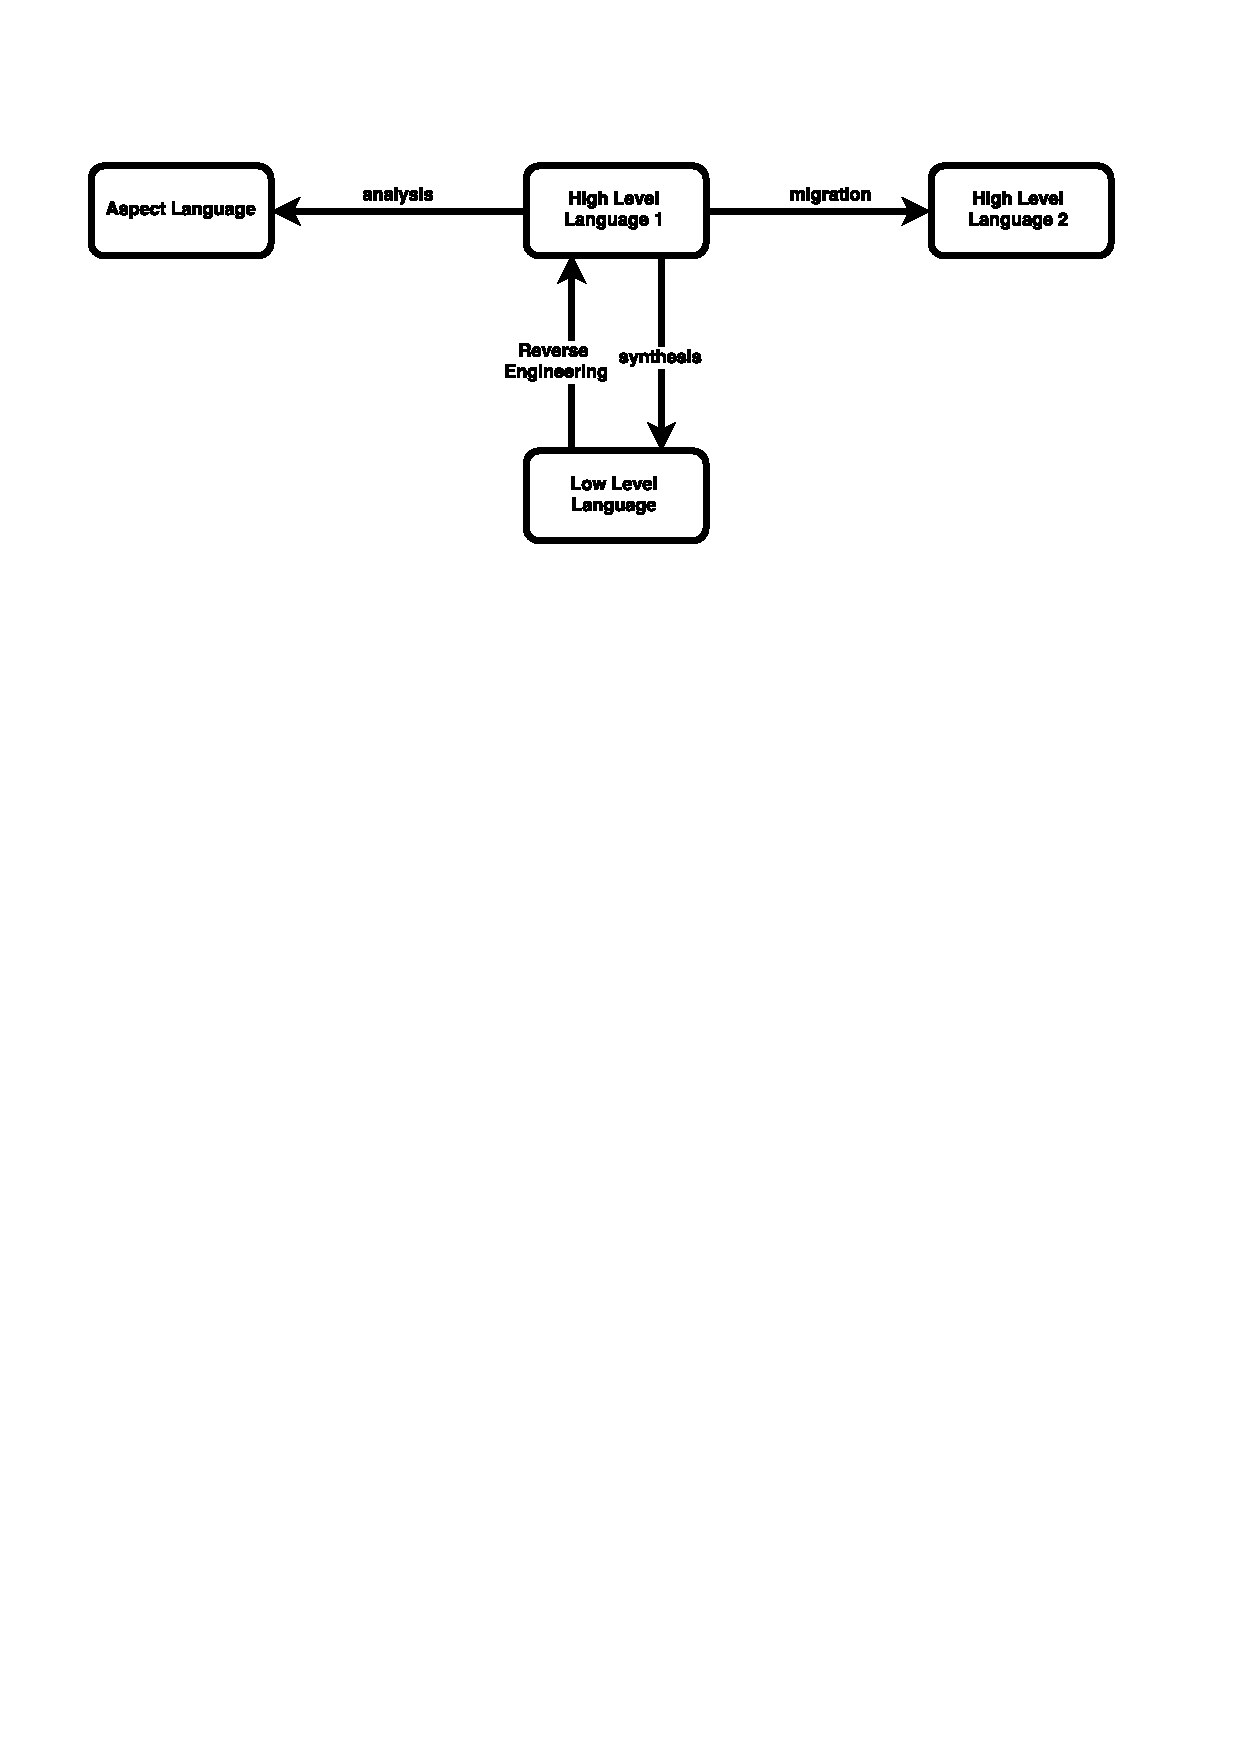
\includegraphics[trim=0.0cm 0.0cm 0.0cm 0.0cm, scale=0.9]{pdf/Taxonomy.pdf}
\vspace{-14.5cm}
\caption{Scenarios of translation}
\label{fig:taxonomy}
\end{figure}
Apart from monitoring the execution of the code, 
static or dynamic analysis can filter,
rewrite and wraps the code inorder to enforce some integrity 
constraints on the code.
The main idea behind the code transformation is to
compute publicly by replacing
all the secret values with dummy variable. Then run the secret computation
under the restrictions. Code transformation is an operation that generates
another program which is semantically equivalent to the original code with
respect to the formal semantics. But sometimes the transformed code can result
to be different from the original code~\cite{Ward:code}. 
This transformation can be done 
manually or using transformation systems. This can be specified as procedures
that are automated which can modify the data structures like abstract syntax tree
in which each statement in the source code is represented as a node in the 
abstract syntax tree. This program transformation
requires effective processing of programs written in any of
the existing programming language.

\chapter{Related Work}
\label{chapter:related}